\documentclass[12pt,a4paper]{article}
\usepackage[UTF8]{ctex}
\usepackage{amsmath,amssymb,amsfonts}
\usepackage{graphicx}
\usepackage{subcaption}
\usepackage{booktabs}
\usepackage{multirow}
\usepackage{multicol}
\usepackage{xcolor}
\usepackage{hyperref}
\usepackage[ruled,vlined]{algorithm2e}



% 设置页边距
\usepackage[top=2.5cm, bottom=2.5cm, left=3cm, right=2.5cm]{geometry}

% 设置行间距
\renewcommand{\baselinestretch}{1.5}

\begin{document}

\title{StructDiT: Zero-Shot Generative Parameter Adaptation for Wireless Communications}
\author{Your Name}
\date{\today}

\maketitle


\begin{abstract}
部署在无线通信系统中的深度学习模型，在分布外（OOD）的信道环境下往往面临严重的性能退化。由于缺乏真实标签、不可接受的延迟以及严格的内存限制，传统的在线微调对于用户设备（UE）而言在根本上是不切实际的。在本文中，我们提出了 \textbf{StructDiT}，这是一个零样本生成式参数自适应框架，它通过条件扩散 Transformer (DiT) 直接合成目标低秩自适应（LoRA）权重，从而绕过了梯度微调。打破了传统直接拼接条件的范式，StructDiT 采用了一个与扩散模型联合训练的 Perceiver Resampler。这种交叉注意力机制能够从 SVD 压缩的带内数据中动态查询最相关的特征，有效地将高维条件（如大规模 MIMO CSI）的复杂性与生成模型的计算负载解耦。为了保持参数空间中的拓扑连贯性，我们将多层 LoRA 矩阵转化为统一的 token 序列，并引入了新颖的结构感知位置编码（层 ID 和矩阵 ID）来显式指导合成过程。此外，针对权重空间固有的“一对多”模糊性问题，我们提出了一种严格的权重规范化机制，打破了排列和符号对称性。结合用于稳定训练收敛的 Min-SNR 权重、用于提升生成保真度的无分类器引导（CFG），以及实现 20 倍推理加速的 DDIM 采样，StructDiT 实现了 SOTA 的零样本泛化能力，在满足严格的实时通信约束的同时，达到了与全量经验训练相媲美的性能。
\end{abstract}


\section{引言}
\label{sec:intro}

% --- Paragraph 1: 背景与核心挑战 ---
随着无线通信向智能化6G演进，超低时延与海量连接成为核心需求。在多输入多输出（MIMO）系统的信道估计与压缩反馈等任务中，常采用基站（BS）与用户设备（UE）分离的深度学习编解码架构。在大规模宏场景中，BS侧的编码器通常保持固定；但UE在面临环境异质性（environmental heterogeneity）而频繁切换微场景时，受地理分布与建筑遮挡等因素影响，其接收特征分布会发生显著变化。这种固定的BS端与动态的UE环境之间深刻的非对称性，会导致预训练的UE解码器在跨域时产生严重的领域偏移与性能衰退。因此，在保持BS端固定且不引入高昂计算开销的前提下，如何为不同微场景中的UE实现灵活、低成本的模型适配，已成为亟待解决的关键问题。

% --- Paragraph 2: 传统泛化方法 ---
针对领域偏移导致的性能下降，无线通信领域已提出多种缓解策略。数据驱动方法试图通过扩充训练集提升泛化能力~\cite{wen2018csinet}，但难以穷举复杂多变的潜在微场景；模型驱动方法利用领域知识人工设计鲁棒特征~\cite{he2019model}，面对全新未知环境时却缺乏动态自适应能力。此外，域适应如 DDA-Net~\cite{feng2023ddanet}通过对齐特征分布促进模型迁移，而元学习~\cite{zhao2025enhanced}则旨在寻找仅需极少样本即可快速收敛的初始化参数。然而，这些传统的跨场景适配机制不仅依赖目标场景的数据收集，且仍需在 UE 端进行昂贵的在线梯度更新，显然难以满足开箱即用的零样本（Zero-Shot）泛化与极低开销的迫切需求。

% --- Paragraph 3: 参数生成范式 ---
鉴于传统跨场景适配机制的固有局限性，本文转向一种新兴范式——参数生成（Parameter Generation）。近年来，参数生成技术在计算机视觉与自然语言处理领域展现出了强大的零样本（Zero-Shot）与跨任务泛化能力。其核心思想是根据特定任务的输入条件动态生成对应的模型参数，从而彻底取代繁琐的模型微调过程~\cite{wang2024neural}。然而，传统面向视觉或语言领域的参数生成方法往往致力于合成包含数千万参数的完整网络权重，其极高的计算开销使其难以直接部署在资源严重受限的 UE 设备上。与此同时，在无线通信领域，近期也有少量初步研究尝试将超网络等参数生成技术应用于信道估计或波束赋形任务~\cite{liu2025hypernetwork}。但遗憾的是，这些方法要么在推理阶段仍需依赖 UE 端的在线微调来寻找最优的条件输入，要么假设 BS 与 UE 具备对等的计算能力并进行联合参数更新。这种机制显然违背了本文所重点关注的“BS 编码器固定、UE 解码器低成本动态切换”的实际非对称通信场景的低价与快速适配。  

% --- Paragraph 4: 方法概述 (PRDiT) ---
为了打破传统跨场景适配机制在计算开销与在线微调上的瓶颈，并有效解决一基站多用户（1-BS-to-multi-UE）场景下的泛化矛盾，本文提出了一种轻量级、即插即用的条件参数生成架构——PRDiT（Perceiver Resampler Diffusion Transformer）。不同于生成庞大的完整解码器网络，PRDiT 首次探索利用条件扩散模型（Conditional Diffusion Models）的强大分布拟合能力，在保持 BS 编码器与 UE 预训练基座固定的前提下，仅根据目标微场景的先验条件动态生成极其轻量化的低秩自适应（LoRA）模块权重。具体而言，针对环境异质性与高维信道特征冗余，预处理条件时先采用奇异值分解（SVD）将 BS 端输出的原始信道特征高效压缩并映射为固定维度的潜在条件表示（Latent Condition Representation）。训练时端到端的 Perceiver Resampler 从潜在条件提取关键特征；Diffusion Transformer（DiT）结构与 AdaLN-Zero 调制机制，使模型能够根据该条件精准生成 UE 解码器前馈网络（FFN）层的 LoRA 权重。同时，为克服神经网络权重空间固有的排列与符号对称性（Permutation and Sign Symmetries），本文还提出了一种基于能量排序（Energy Sorting）与符号翻转（Sign Flipping）的权重规范化（Canonicalization）策略对权重进行规范化，极大提升了生成过程的稳定性与一致性。凭借这种创新设计，UE 设备无需存储多个专用解码器，也彻底免去了设备端的梯度更新负担，在面临微场景切换时能够以极低的额外计算成本实现通信性能的开箱即用与快速恢复。


为打破传统跨场景适配方法在计算开销与在线微调上的瓶颈，并有效解决一基站多用户（1-BS-to-multi-UE）场景下的泛化矛盾，本文提出了一种轻量级、即插即用的条件参数生成架构——PR-DiT（Perceiver Resampler Diffusion Transformer）。该架构利用条件扩散模型，在保持 BS 编码器与 UE 基座固定的前提下，直接根据目标微场景先验，动态生成 UE 解码器前馈网络（FFN）的低秩自适应（LoRA）权重。在宏观执行流上，条件预处理阶段首先利用奇异值分解（SVD）将高维冗余的信道特征压缩为紧凑的潜在条件；随后，由 Perceiver Resampler 提取关键特征，引导结合 AdaLN-Zero 调制的 DiT 网络精准合成参数。同时，为消除神经网络权重固有的排列与符号对称性，本文引入了基于能量排序与符号翻转的规范化（Canonicalization）策略，确保了生成目标的一致性与稳定流形。凭借这一创新，UE 设备彻底免去了本地梯度更新负担与多模型存储开销，在面临微场景切换时能够以极低代价实现开箱即用的通信性能恢复。

% --- Paragraph 5: Contributions ---
本文的主要贡献总结如下：

\begin{itemize}
    \item \textbf{新视角}
    系统性研究了无线通信中“BS 固定、UE 变化”范式下的模型泛化问题，并首次将高效参数生成技术引入该无线通信领域，为解决固定 BS 编码器与动态 UE 环境之间的泛化矛盾提供了一种新的研究视角。

    \item \textbf{方法设计}
    提出高效的 PRDiT 参数生成架构，通过引入 SVD 条件降维、Perceiver Resampler 以及权重 Canonicalization 等策略，显著降低参数生成的计算复杂度。相比传统微调或多模型集成方法，该方法具有更高的计算效率，能够满足通信系统对低时延的需求。

    \item \textbf{实验验证}
    在标准无线通信数据集 DeepMIMO 和 WAIRD 上进行了大量实验，结果表明所提出的方法在跨场景 CSI 压缩反馈与信道估计任务中显著提升了模型泛化性能，同时其推理与参数生成开销明显低于传统微调方法以及大型生成模型基线。
\end{itemize}


\section{Preliminary}
\label{subsec:preliminaries}

\subsection*{Low-Rank Adaptation (LoRA)}
在非对称的无线通信部署场景中，为避免在资源受限的用户设备（UE）端进行全量参数更新，本文采用低秩自适应（Low-Rank Adaptation, LoRA）\cite{hu2021lora} 作为轻量化适配方案。LoRA 的核心思想是冻结预训练解码器的原始权重矩阵 $W_0 \in \mathbb{R}^{d \times k}$，并在旁路引入两个可分解的低秩矩阵进行参数更新：降维矩阵 $A \in \mathbb{R}^{r \times k}$ 和升维矩阵 $B \in \mathbb{R}^{d \times r}$，其中秩 $r \ll \min(d, k)$。修改后的前向传播表示为：
\begin{equation}
W_0 x + \Delta W x = W_0 x + B(A x)
\end{equation}
由于环境异质性，不同微场景需要不同的 LoRA 权重。在此架构中，参数矩阵 $A$（较小的矩阵）和 $B$（较大的矩阵）将被展平为 Token 序列。本文的目标不再是通过传统的梯度下降微调这些参数，而是将其作为连续分布空间中的目标流形，通过生成式模型直接合成特定于各个层（layer\_ids）和矩阵类型（matrix\_ids）的 LoRA 参数。

\subsection*{Conditional Diffusion Models and Guidance}
本文利用条件扩散模型（Conditional Diffusion Models）学习从目标环境的潜在特征 $c$ 到 LoRA 权重参数空间的映射。给定高质量的真实参数数据 $x_0$，扩散模型通过参数化马尔可夫链定义了前向加噪与反向去噪过程。

\textbf{前向过程（Forward Process）：} 前向过程在给定时间步 $t \in [1, T]$ 下逐步向参数 $x_0$ 添加高斯噪声。设 $\beta_t$ 为噪声调度的方差，定义 $\alpha_t = 1 - \beta_t$ 以及累积乘积 $\bar{\alpha}_t = \prod_{s=1}^t \alpha_s$，任意时间步 $t$ 的边缘分布可直接写为：
\begin{equation}
q(x_t | x_0) = \mathcal{N}(x_t; \sqrt{\bar{\alpha}_t} x_0, (1 - \bar{\alpha}_t)\mathbf{I})
\end{equation}
这允许我们利用重参数化技巧直接从 $x_0$ 采样 $x_t = \sqrt{\bar{\alpha}_t} x_0 + \sqrt{1 - \bar{\alpha}_t}\epsilon$，其中 $\epsilon \sim \mathcal{N}(0, \mathbf{I})$。

\textbf{反向过程（Reverse Process）：} 反向过程旨在给定环境条件 $c$ 下，从纯高斯噪声 $x_T$ 中逐步去噪重建网络权重。该过程被建模为由神经网络参数化的高斯转移：
\begin{equation}
p_\theta(x_{t-1} | x_t, c) = \mathcal{N}(x_{t-1}; \mu_\theta(x_t, t, c), \Sigma_\theta(x_t, t, c))
\end{equation}
其中，去噪网络 $\theta$（本文采用 Diffusion Transformer, DiT）通过观察带噪序列 $x_t$、时间步 $t$ 及环境条件 $c$ 来预测去噪目标。以预测噪声 $\epsilon$ 为例，基础的去噪目标函数可统一表示为：
\begin{equation}
L_{simple} = \mathbb{E}_{x_0, \epsilon, c, t} \left[ \| \text{Target} - D_\theta(x_t, t, c) \|_2^2 \right]
\end{equation}

\textbf{无分类器引导（Classifier-Free Guidance, CFG）：}
为进一步增强条件 $c$ 对参数生成的控制力并提升跨场景一致性，本文引入了无分类器引导机制。在训练阶段，模型以一定的概率将输入条件 $c$ 替换为可学习的无条件表示（Null Condition, $\emptyset$）。在推理阶段，通过外推有条件预测与无条件预测的差异，即可对生成方向进行强化引导：
\begin{equation}
\tilde{D}_\theta(x_t, t, c) = D_\theta(x_t, t, \emptyset) + s \cdot \left( D_\theta(x_t, t, c) - D_\theta(x_t, t, \emptyset) \right)
\end{equation}
其中 $s \ge 1.0$ 为引导缩放系数。这种机制使得生成的 LoRA 参数能够高度敏锐地适配给定的微场景信道特征。


\section{Methodology}
\label{sec:method}

\subsection{Problem Formulation and PR-DiT Overview}
\label{subsec:overview}
\textbf{问题定义.} 在非对称的无线通信部署场景中，一基站多用户（1-BS-to-multi-UE）架构面临着严峻的泛化挑战。假设基站端的预训练编码器固定为 $f_{\text{enc}}$，用户（UE）端预训练解码器的主干参数固定为 $\Phi_0$。对于任意异质的未知微场景 $\mathcal{S}$，给定输入信号 $X$，编码特征为 $Z = f_{\text{enc}}(X)$。为了克服领域偏移，传统自适应方法需要在 UE 端引入 LoRA 权重 $W = \{A_1, B_1, A_2, B_2\}$，并通过在线反向传播求解特定场景的最优参数 $W^*_{\mathcal{S}}$：
\begin{equation}
W^*_{\mathcal{S}} = \arg\min_{W} \mathbb{E}_{(X, Z) \sim \mathcal{S}} \left[ \mathcal{L}_{\text{task}} \big( f_{\text{dec}}(Z; \Phi_0, W), X \big) \right]
\end{equation}
其中 $\mathcal{L}_{\text{task}}$ 为信道估计或压缩反馈的重构损失。然而，在资源受限的 UE 端求解上式会带来高昂的计算与时延开销。因此，本文的目标是彻底规避在线优化过程，转而学习一个条件参数生成模型 $p_\theta(W | c)$，通过单次前向推理直接从连续流形中采样出高度适配的参数，即 $\hat{W} \sim p_\theta(W | c) \approx W^*_{\mathcal{S}}$。

在构建生成条件 $c$ 时，由于 $f_{\text{enc}}$ 输出的原始信道特征 $Z$ 维度极高且包含大量冗余与环境噪声，直接将其注入生成模型会导致严重的维度灾难（Dimensionality Curse）与显存溢出。因此，在 PR-DiT 框架中，我们首先引入奇异值分解（SVD）对高维特征 $Z$ 进行无监督提纯：
\begin{equation}
c = \text{SVD}_{\text{trunc}}(Z) \in \mathbb{R}^{224 \times 512}
\end{equation}
该操作提取了表征当前物理信道最核心的主成分，将其作为高度紧凑的环境先验条件 $c$。

基于上述数学定义，PR-DiT 开创性地提供了一种端到端的条件参数生成 Pipeline。在训练阶段，UE 端离线收集的真实 LoRA 权重 $W^*_{\mathcal{S}}$ 经过规范化（Canonicalization）后展平为一维 Token 序列并逐步加噪；Perceiver Resampler 通过交叉注意力从压缩条件 $c$ 中提取定长特征；随后，DiT 以该特征为条件引导，逐步从高斯噪声中去噪预测真实的权重 Token。在推理阶段，面对未知通信场景，PR-DiT 仅需提取当前条件 $c$，前向采样生成 Token，经反规范化重组后即插即用至 UE 端解码器，实现零样本泛化。

\subsection{Parameter Space Canonicalization}
\label{subsec:canonicalization}
神经网络权重空间固有的排列对称性（Permutation Symmetry）和符号模糊性（Sign Ambiguity）会导致严重的一对多映射问题。若不加以消除，扩散模型在拟合分布时会将不同排列的等效权重平均化，导致生成失效。为此，我们提出一种规范化对齐策略\ref{alg:canonicalization}，旨在完全保持 LoRA 原有表示能力的前提下，为扩散模型提供唯一且确定的目标流形。

\textbf{Mathematical Invariance.} 
为了证明规范化操作不会改变预训练 LoRA 模块的前向映射逻辑，我们将核心权重乘积 $\Delta W = BA$ 等价展开为 $r$ 个秩为 1 的矩阵之和：
\begin{equation}
\Delta W = BA = \sum_{i=1}^{r} b_i a_i^T
\end{equation}
其中 $a_i^T \in \mathbb{R}^{1 \times k}$ 和 $b_i \in \mathbb{R}^{d \times 1}$ 分别为降维矩阵 $A$ 的行向量与升维矩阵 $B$ 的列向量。针对两种模糊性，我们的策略及等价性推导如下：

\begin{itemize}
    \item \textbf{排列等价性（Permutation Invariance）：} 我们计算各秩分量的“能量”（范数乘积 $\|a_i\| \cdot \|b_i\|$）并强制其降序重排。通过引入置换矩阵 $P \in \{0,1\}^{r \times r}$（满足 $P^T P = I$），该重排操作可表示为 $\tilde{B}\tilde{A} = (BP^T)(PA) = B(P^TP)A = BA$，从根本上不改变 $\Delta W$。
    
    \item \textbf{符号等价性（Sign Invariance）：} 我们以重排后 $A$ 中各行绝对值最大元素的符号为基准，对 $A$ 和 $B$ 的对应分量进行符号翻转。引入对角符号矩阵 $S = \text{diag}(s_1, \dots, s_r)$ 且 $s_i \in \{-1, 1\}$，由于 $S^2 = I$，更新量变为 $\tilde{B}\tilde{A} = (BS)(SA) = BS^2A = BA$。
\end{itemize}

经过上述规范化操作后，我们对四组权重矩阵（$A_1, B_1, A_2, B_2$）执行全局均值-标准差归一化，从而平滑高维参数空间，稳定扩散模型的训练过程。

\begin{algorithm}[htpb]
\caption{LoRA Parameter Canonicalization}
\label{alg:canonicalization}
\KwIn{LoRA weight matrices $A \in \mathbb{R}^{r \times k}$ and $B \in \mathbb{R}^{d \times r}$.}
\KwOut{Canonicalized weight matrices $\tilde{A}$ and $\tilde{B}$.}
\tcp{Step 1: Compute Energy and Sort (Resolve Permutation Ambiguity)}
Compute row norms for $A$: $u \leftarrow (\|a_1\|_2, \|a_2\|_2, \dots, \|a_r\|_2)$\;
Compute column norms for $B$: $v \leftarrow (\|b_1\|_2, \|b_2\|_2, \dots, \|b_r\|_2)$\;
Compute energy score for each rank: $E \leftarrow u \odot v$\;
Obtain sorted indices in descending order: $\text{idx} \leftarrow \text{argsort}(E, \text{descending}=\text{True})$\;
Permute matrices: $A' \leftarrow A[\text{idx}, :]$, $B' \leftarrow B[:, \text{idx}]$\;

\tcp{Step 2: Sign Flipping (Resolve Sign Ambiguity)}
Find indices of elements with max absolute value in each row of $A'$: 
$\text{idx}_{\max} \leftarrow \text{argmax}(|A'|, \text{dim}=1)$\;
Extract the signs of these elements: 
$S \leftarrow \text{sign}\left( A'[\text{range}(r), \text{idx}_{\max}] \right)$\;
\For{$i = 1$ \KwTo $r$}{
    \If{$S[i] == 0$}{
        $S[i] \leftarrow 1$ \tcp*{Handle edge case of exact zero}
    }
}
Apply sign flipping: $\tilde{A} \leftarrow \text{diag}(S) A'$ and $\tilde{B} \leftarrow B' \text{diag}(S)$\;
\Return{$\tilde{A}, \tilde{B}$}
\end{algorithm}

\subsection{Conditional Generation}
\label{subsec:architecture}

\subsubsection*{Conditioning via Perceiver Resampler}
尽管信道特征已通过 SVD 降维，但直接作为条件序列送入 DiT 仍会带来显著的计算开销。受感知器架构启发，本文引入可端到端训练的 Perceiver Resampler 作为条件编码器。我们初始化一组固定数量的可学习潜在查询向量（Latent Queries），通过交叉注意力机制（Cross-Attention）主动从复杂的 SVD 特征中提取关键的物理传播特征，将其进一步压缩为固定维度的潜在嵌入（Latent Embeddings）。该机制有效解耦了输入条件的维度复杂度与生成主干的计算量。此外，在训练时我们向提取的条件特征中注入微量随机噪声，进一步增强了模型对抗信道估计误差的鲁棒性。
 
\subsubsection*{Structure-Aware Diffusion Transformer}
本文采用 Diffusion Transformer (DiT) 作为去噪网络 $\epsilon_\theta$。由于经过展平的 LoRA 矩阵失去了原本的二维结构属性，我们专门设计了结构位置编码（Structure Embeddings）。除了标准的序列正弦位置编码，我们额外引入了层索引（Layer ID Embedding）和矩阵类型索引（Matrix ID Embedding），显式地将 Token 的物理拓扑信息（Linear 1/2，$A$/$B$）注入模型，使 DiT 能够精准感知各 Token 在高维参数流形中的局部与全局语义。

在条件注入方面，我们采用自适应层归一化（AdaLN-Zero）调制机制。在每个 DiT 模块中，扩散时间步 $t$ 与 Resampler 提取的条件嵌入被融合，并回归为 AdaLN 的缩放（Scale）与平移（Shift）参数。特别是，我们将每个模块最后一层 MLP 与 AdaLN 的调制参数初始化为零，使模型在训练初期表现为恒等映射（Identity Function），极大地加速了网络收敛并确保了极深 Transformer 的训练稳定性。

\subsection{Optimization Objective and Inference}
\label{subsec:optimization}
在训练扩散模型时，直接采用标准的全局均方误差（MSE）损失往往难以应对参数生成任务中的尺度不均与噪声震荡问题。为此，本文设计了融合尺寸感知（Size-Aware）与 Min-SNR 截断的复合优化目标。

\textbf{Size-Aware Loss Weighting.} LoRA 模块中降维矩阵 $A \in \mathbb{R}^{r \times k}$（小矩阵）和升维矩阵 $B \in \mathbb{R}^{d \times r}$（大矩阵）的参数量差异可达数个数量级。若无差别计算损失，大矩阵产生的庞大梯度会完全淹没小矩阵的特征学习。设 $x_t$ 为时间步 $t$ 的带噪 token 序列，$\epsilon$ 为添加的真实高斯噪声，$\hat{\epsilon}$ 为网络预测的噪声。我们利用预先构建的结构索引生成布尔掩码 $M_{\text{small}}$ 和 $M_{\text{large}}$，将全局损失进行解耦：
\begin{equation}
\mathcal{L}_{\text{small}} = \frac{1}{|M_{\text{small}}|} \sum_{i \in M_{\text{small}}} \|\epsilon_i - \hat{\epsilon}_i\|_2^2
\end{equation}
\begin{equation}
\mathcal{L}_{\text{large}} = \frac{1}{|M_{\text{large}}|} \sum_{j \in M_{\text{large}}} \|\epsilon_j - \hat{\epsilon}_j\|_2^2
\end{equation}
引入平衡超参数 $w_s \in (0, 1)$，我们构建了加权内部损失 $\mathcal{L}_{\text{batch}} = w_s \mathcal{L}_{\text{small}} + (1 - w_s) \mathcal{L}_{\text{large}}$，从而赋予小矩阵更高的相对优化权重。

\textbf{Min-SNR Weighting and CFG.} 为解决扩散过程早期（$t \to T$，极度嘈杂阶段）预测难度极大导致的梯度震荡，我们引入信噪比（SNR）截断权重 $\lambda(t) = \min(\text{SNR}(t), \gamma)$。同时，为支持无分类器引导（CFG），我们以概率 $p_{\text{drop}}$ 将条件 $c$ 替换为可学习的无条件嵌入 $\emptyset$。最终的完整优化目标定义为：
\begin{equation}
\mathcal{L}_{\text{ours}} = \mathbb{E}_{x_0, \epsilon, c, t} \left[ \lambda(t) \cdot \mathcal{L}_{\text{batch}}(x_t, t, c_{\text{drop}}) \right]
\end{equation}

\textbf{Inference.} 在推理部署阶段，面对无线通信系统严格的时延限制，传统的长序列马尔可夫采样难以满足即插即用的需求。为此，本文采用非马尔可夫的 DDIM（Denoising Diffusion Implicit Models）加速采样算法，通过确定性生成机制，将反向去噪过程从通常的 1000 步大幅压缩至 50 步以内。

在采样过程中，为显式强化微场景条件 $c$ 对生成参数流形的引导力，我们利用无分类器引导（CFG）对外推噪声 $\tilde{\epsilon}_\theta$ 进行了尺度校准：
\begin{equation}
\tilde{\epsilon}_\theta(x_t, t, c) = \epsilon_\theta(x_t, t, \emptyset) + s \cdot \big( \epsilon_\theta(x_t, t, c) - \epsilon_\theta(x_t, t, \emptyset) \big)
\end{equation}
其中引导尺度 $s \ge 1.0$ 用于在生成参数的多样性与当前信道环境的契合度之间进行灵活权衡。

此外，为消除训练末期梯度更新带来的局部参数震荡，推理阶段统一调用网络权重的指数移动平均（EMA）版本。其平滑更新规则为 $\theta_{\text{EMA}} = m \theta_{\text{EMA}} + (1 - m) \theta$。凭借 DDIM 极速采样与 EMA 平滑策略，PR-DiT 能够以极低的额外计算开销，稳定、极速地解码出高质量的自适应 LoRA 参数流形。


\section{Experiment}
In this section, we first show the experiment setup. Then, we present the evaluation results, ablation studies, and analysis of PR-DiT.

\subsection{Experiment setup}
\label{subsec:data_prep}

\paragraph{Datasets and metrics.}
本文在实验中采用了均包含上百个复杂的通信微场景的 WAIRD~\cite{wang2022waird} 以及 DeepMIMO~\cite{alkhateeb2019deepmimo}进行压缩反馈或信道估计。为了定量评估模型在跨场景下的信道估计与 CSI 压缩反馈性能，我们统一采用归一化均方误差（Normalized Mean Squared Error, NMSE）作为核心评价指标。

\paragraph{Parameter \& condition collecting.}
我们用 10\% 的场景数据预训练 Transformer 基座模型（含 BS 编码器与 UE 解码器）。随后冻结主干网络，在剩余目标微场景中，仅对 UE 解码器前馈网络（FFN）层的 LoRA 模块进行特异性微调，并提取收敛后的 LoRA 权重作为目标生成参数。同时，我们提取对应场景下固定 BS 编码器的输出特征并采用奇异值分解（SVD）将其降维为 $224 \times 512$ 的紧凑潜在矩阵\ref{fig:svd_comparison}作为环境引导条件。最终建出大规模的 $\langle \text{压缩信道特征}, \text{LoRA权重} \rangle$ 数据对，作为扩散模型的训练数据。

\begin{figure}[htbp]
    \centering
    % 左侧原始高维矩阵图
    \begin{subfigure}[b]{0.45\textwidth}
        \centering
        \includegraphics[width=\textwidth]{./figures/heatmap_raw.png}
        \caption{Original High-Dimensional Feature}
        \label{fig:orig_matrix}
    \end{subfigure}
    \hfill % 添加弹性间距，让两张图推向两边
    % 右侧 SVD 压缩后的矩阵图
    \begin{subfigure}[b]{0.45\textwidth}
        \centering
        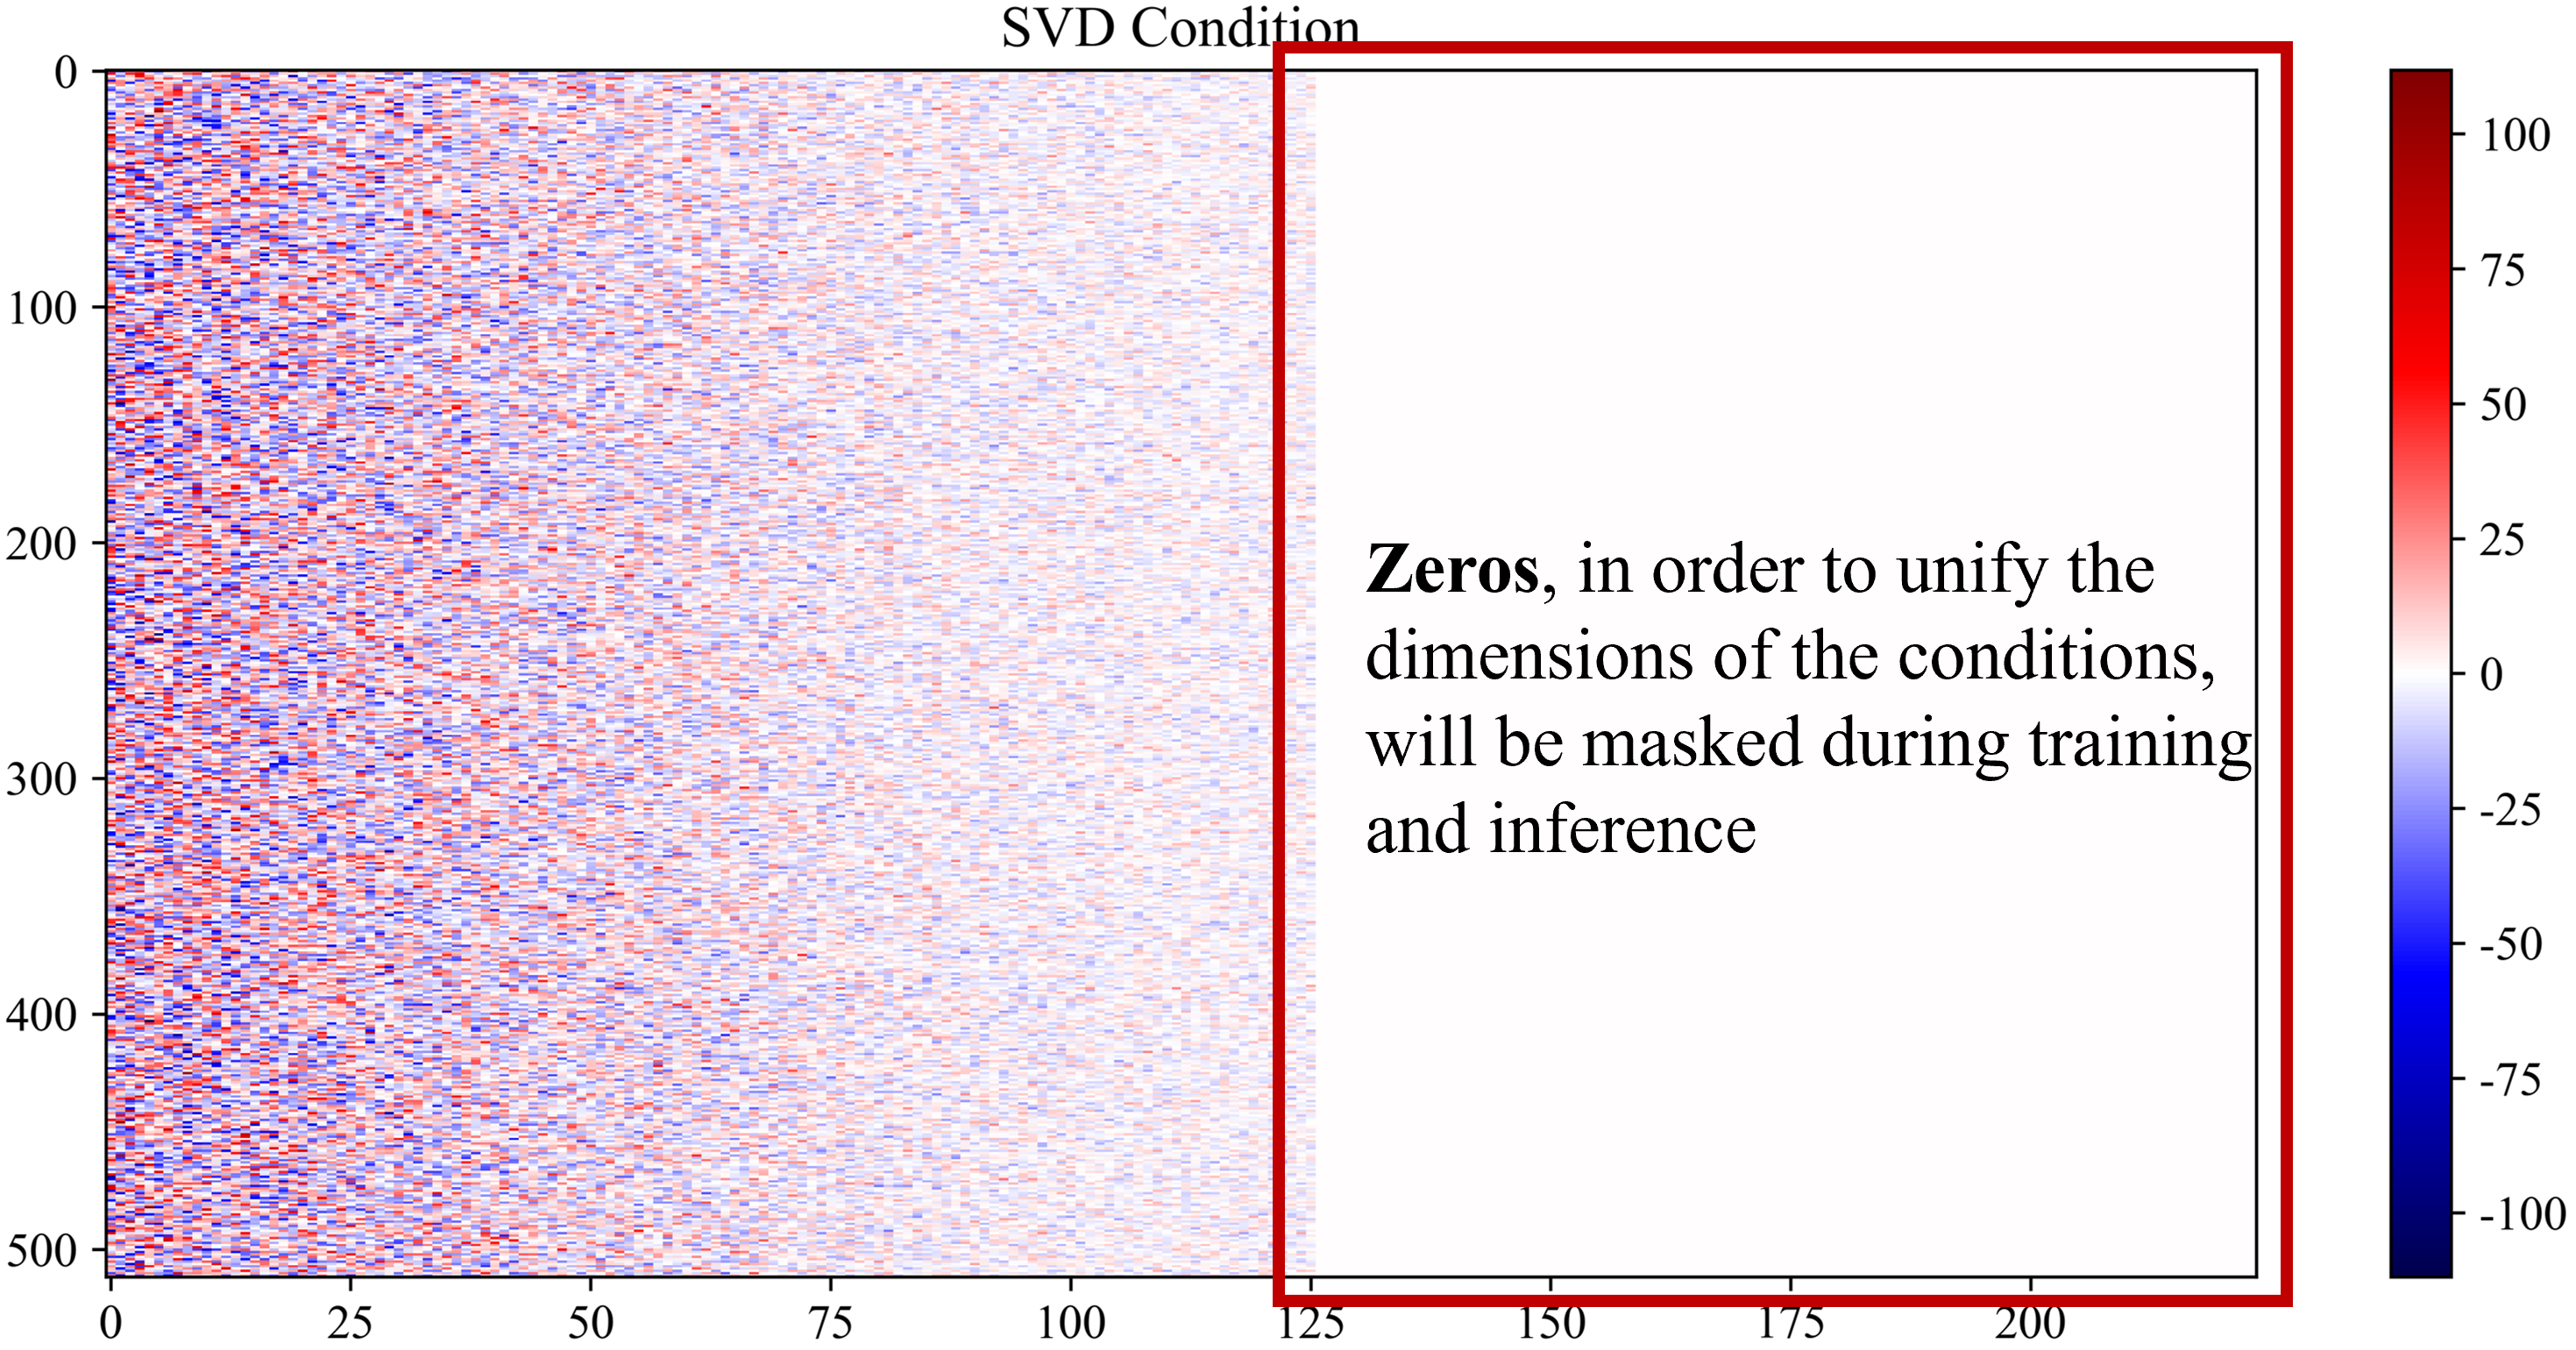
\includegraphics[width=\textwidth]{./figures/heatmap_svd.png}
        \caption{SVD-Compressed Latent Feature}
        \label{fig:svd_matrix}
    \end{subfigure}
    \caption{Comparison of the channel feature feature before and after SVD compression.}
    \label{fig:svd_comparison}
\end{figure}


\section{Related Work}

\subsection{传统无线通信领域的泛化性}
在大规模 MIMO 系统中，深度学习模型在部署到具有不同几何分布的用户设备（UE）时，会遭遇严重的领域偏移。早期的数据驱动方法主要通过扩充训练数据集以期覆盖更多场景 \cite{wen2018csinet, guo2020overview, jin2021transnet, mashhadi2020pruning, sun2022generalization}，但由于实际无线环境的电磁传播特性极为复杂且不可预测，几乎不可能穷举所有潜在的信道状态。为了提升鲁棒性，旨在利用通信物理层先验知识来约束深度学习模型特征表示的模型驱动方法被提出 \cite{he2019model}，然而这类人工设计的特征在面对未知拓扑时依然缺乏足够的动态自适应能力。为了更系统地缓解这种泛化差距，学术界引入了试图对齐源域和目标域特征分布的域适应机制 \cite{feng2023ddanet, da2025_mimo, da2025_doa}，以及旨在学习高泛化性初始化参数的元学习和迁移学习范式 \cite{finn2017model, lu2021transfer, yuan2021meta, park2021meta, zhao2025enhanced, meta2025_csi, knowledge_meta2024}。尽管如此，这些传统缓解方法大多存在两个致命缺陷：一是严重依赖目标场景的离线数据收集，二是仍需在计算资源受限的 UE 端进行在线梯度更新 \cite{generalizable2025_csi, transfer2024_online}，这些令人望而却步的计算开销直接阻碍了真正即插即用式的零样本（Zero-Shot）泛化。

\subsection{参数生成领域的泛化性}
鉴于传统跨域适配机制在计算范式上的固有局限，建立从输入条件直接映射到神经网络权重分布连续流形的参数生成（Parameter Generation）作为一种新兴范式，正展现出极具潜力的零样本泛化能力，其能在推理阶段彻底取代繁琐且高成本的模型微调过程 \cite{ha2016hypernetworks}。近年来，基于生成式先验的参数生成技术在计算机视觉与自然语言处理领域取得了突破性进展，特别是扩散模型 \cite{ho2020denoising, peebles2023diffusion, peebles2022learning} 和流匹配架构 \cite{flowmatch2025_dynamics}，已被证明能在无梯度优化的前提下为未见拓扑和目标分布合成任务特异性的网络参数 \cite{wang2024neural, zhang2023neural, nnit2026_diffusion, d2nwg2025}。此外，基于条件提示的生成器通过将解耦后的条件直接映射为低秩自适应（LoRA）权重 \cite{hu2021lora}，显著降低了生成维度的压力并展现出极强的跨域鲁棒性 \cite{dnd2025_llm}。尽管这些方法通过学习条件空间到参数流形的连续映射实现了完全避开反向传播的动态自适应，但传统面向视觉或语言领域的参数生成往往致力于合成包含数千万参数的完整网络权重，极高的计算开销使其难以直接部署在资源严重受限的边缘设备上。

\subsection{无线系统中的参数生成}
在无线通信领域，初步的研究已经开始探索利用参数生成技术来提供环境适应性，当前主流方法多集中于利用传统的超网络（Hypernetworks）为 CSI 反馈 \cite{sun2022hypercsi, hrnet2024}、信道估计 \cite{liu2021deep, liu2025hypernetwork} 以及时变非平稳信道预测 \cite{hyperchannel2024, hyper_ce_2025} 动态生成参数。虽然这些方法在理论上提供了实例级别的灵活性，但在应对跨多个 UE 的宏观空间领域偏移时存在根本性局限：它们大多假设基站（BS）与 UE 具备对等的计算能力并进行联合参数更新，或在推理阶段仍需依赖 UE 端的在线微调来寻找最优条件输入 \cite{liu2025hypernetwork}，严重违背了“BS 端编码固定、UE 端解码低成本动态切换”的实际非对称通信场景需求。其次，简单的超网络生成器在处理高维原始的大规模 MIMO CSI 数据时不可避免地会遭遇维度灾难，且缺乏针对复杂信道环境特征的显式解耦机制。为了填补这一关键空白，本文提出的 PR-DiT 引入了一种全新的 Pipeline：我们利用奇异值分解（SVD）结合感知器重采样（Perceiver Resampler）高效压缩并提取高维信道冗余信息，随后利用扩散 Transformer（DiT）以纯零样本的方式为未见场景生成轻量化的 LoRA 权重，在兼顾低开销的同时实现了极致的环境自适应能力。







\bibliographystyle{plain} % 或者 NeurIPS 要求的格式，如 plainnat
\bibliography{references} % 链接你的 .bib 文件





\end{document}